\chapter{Inventing Color}
\footnote{Written by Sam Usman and Brent Barker, with contributions from Mike
Gladders, Amanda Pagul, and others.}

Everything in the universe glows, giving off electromagnetic waves at in the
form of \emph{thermal radiation} (also called \emph{blackbody radiation}). The
warmer the object, the more radiation the object will give off.
Let's make the rainbow to get idea of how this works
%%FIXME: why doesn't this reference work correctly.
%Figure~\ref{fig:blackbody} shows how the warmer an object is, the brighter it
%will look.
\nopagebreak
%\begin{figure}
%\label{fig:blackbody}
%\centering
%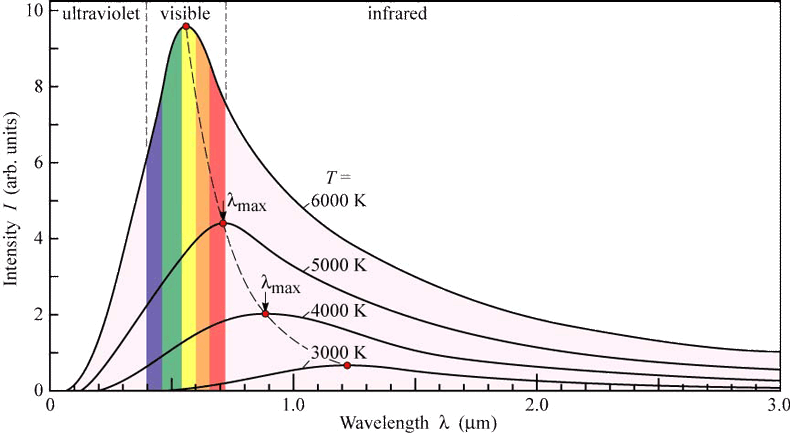
\includegraphics[width=\textwidth]{inventing-color/blackbody.png}[Ht]
%\caption{This figure shows the relationship between light intensity at
%different wavelengths and temperature. The x-axis is wavelength, so high-energy
%light like X-rays are on the left, while low-energy light like infrared is on
%the right. The rainbow represents the part of the spectrum that can be
%perceived by the human eye. Each line represents the intensity for a different
%temperature. Notice how the warmer an object is, the brighter it is at
%\emph{all} wavelengths, and its \emph{peak} intensity is at higher and higher
%frequencies, i.e. moves to the bluer part of the spectrum.} 
%\end{figure}

%%TODO rewrite rgb image directions. these are very unclear.
%
%%TODO for "conduct an experiment", be more clear about what deliverables / product is wanted

The light's intensity $B$ at wavelength $\lambda$ and
temperature $T$ is given by Planck's Law:
%
\begin{equation}
\label{eq:planck}
 B(\lambda, T) = \frac{2 h c^2}{\lambda^5}
 \frac{1}{\exp\left( \frac{hc}{\lambda k_\textrm{B} T} \right) - 1} \,,
\end{equation}
%
Here, $h$ is the Planck constant, $c$ is the speed of light in the medium
(usually assumed to be vacuum), and $k_\textrm{B}$ is the Boltzmann constant.
The \emph{brightest} (peak) wavelength can be calculted using Wien's law:
$\lambda_\textrm{peak}$ is given by Wien's displacement law,
%
\begin{equation}\label{ic:eq:wien}
	\lambda_\textrm{peak} = \frac{b}{T} \,,
\end{equation}
%
Here $b \approx 2898\:\mu$m$\cdot$K is Wien's displacement constant.
This means, we can figure out how hot something is by looking at its peak
wavelength!

\section{Make the rainbow! (But please don't taste the rainbow!)}
\label{ic:sec:exploring}

\begin{steps}
\item\label{ic:step:load-sim} Load the interactive thermal radiation simulation
at
\url{https://phet.colorado.edu/sims/html/blackbody-spectrum/latest/blackbody-spectrum_en.html}

\item Play with the controls and see what happens. Discuss among your team.

\item Find a pattern --- how does the shape change as the temperature goes up? 
For example, how does the peak wavelength change, and how about the total
radiated power (area under curve)? \textbf{Record your observations.}
        
\item At what peak wavelength do you radiate? Use the sim to determine this and 
estimate your uncertainty. \textbf{Record your findings.}

\item Using your estimated temperature, calculate your peak wavelength 
according to Wien's law.

\item\label{ic:step:qual-color} Comparing the spectra of the light bulb, Sun, 
and Sirius A, how can you use the spectrum to determine what color each one
appears as?
\end{steps}

\noindent
\fbox{
\begin{minipage}{0.45\textwidth}
\textbf{Question:}

What is the peak wavelength of light that \emph{humans} give off?  Assume the
average human body temperature is about \~310 K.  Humans can see in the range
of 380 to 700 nanometers (aka $10^{-9}$ m). Does your answer make sense? (If
you are in a dark room, would you be able to spot the human from their glow?)
\textbf{Include this in your lab report.}
\end{minipage}}
\hspace{0.3cm}
\vspace{0.2cm}
\begin{minipage}{0.5\textwidth}
This also means that we can measure the temperature of something really far
away by looking at how bright it is at different wavelengths!

In this lab, we'll simulate this by measuring the radiation that is given off
by a lightbulb at various temperatures.  Then we'll use filters to estimate the
intensity of light at different wavelength ranges.
\end{minipage} 

Then, we'll make a color image by combining colors from different wavelength
ranges!  This is the same method as is used to make beautiful space photos that
we see from NASA and other academic places.

\section{See the rainbow!}
\label{sec:diffraction}
Objects release a very specific range of wavelengths depending on their
temperature, as we can see in Equation~\ref{eq:planck}.
So let's try to do that for ourselves and try to figure out the relationship
between the temperature of an object and its color.

We're going to start by looking at a rainbow coming from a lightbulb. 
\begin{steps}
\item Take one of the diffraction gratings (shown in Figure~\ref{fig:grating}).
Look at the lightbulb with adjustable voltage directly through grating. Then
turn so you're now facing about 30 degrees to the left or the right. (You
\emph{will not} see the lightbulb through the grating anymore, but you
\emph{should} see its light.) 
\end{steps}

\noindent
\fbox{
\begin{minipage}{0.45\textwidth}
\textbf{Question:}
What do you see through the grating? How do you think this would change if you
were viewing different light sources such as: a neon sign? Light from the sun?
A street lamp?
\textbf{Include your response in your lab report.}
\end{minipage}}
\hspace{0.3cm}
\vspace{0.2cm}
\begin{minipage}{0.5\textwidth}
\end{minipage}

\begin{figure}
\label{fig:grating}
       \centering
       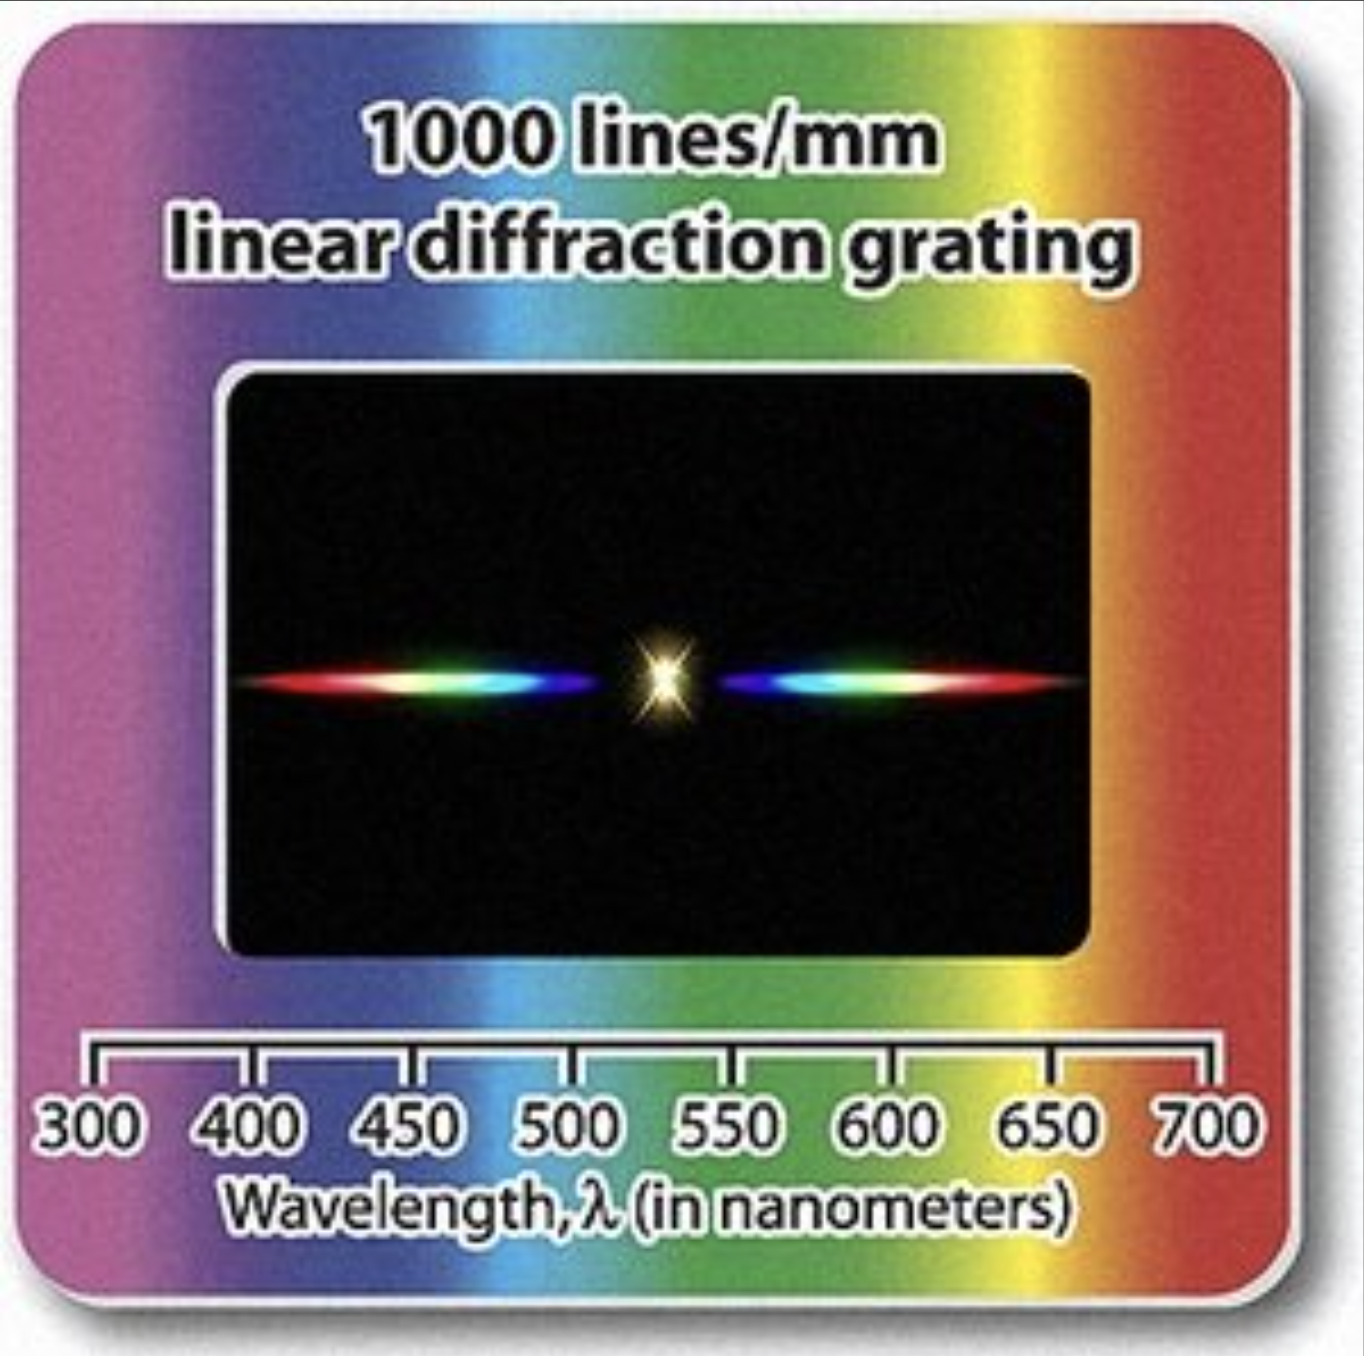
\includegraphics[width=0.2\textwidth]{inventing-color/diffraction.png}
       \caption{Use this grating to observe light from the adjustable voltage lightbulb.}
\end{figure}

\begin{figure}
\label{fig:grating}
       \centering
       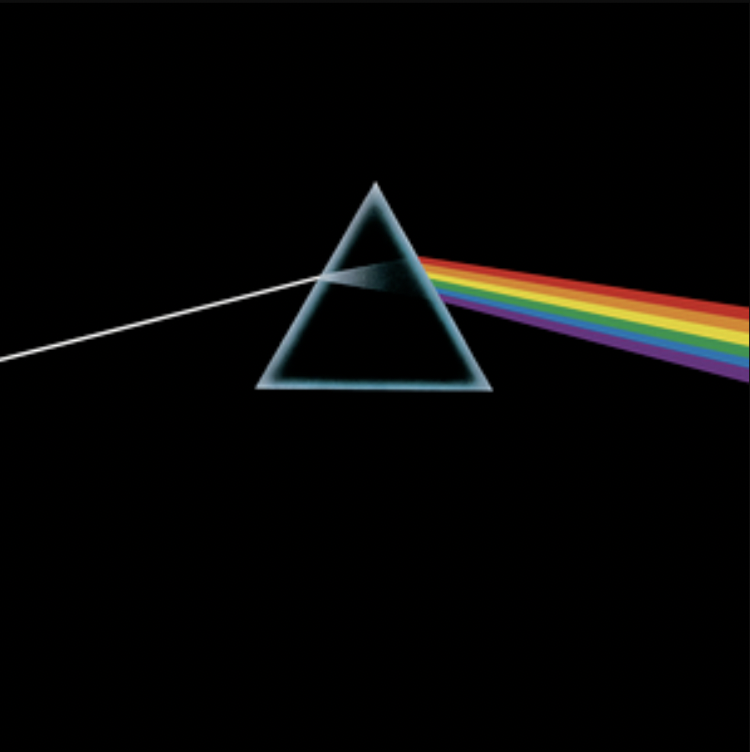
\includegraphics[width=0.5\textwidth]{inventing-color/prism.png}
       \caption{The grating works similarly to a prism: the light is refracted
through the medium, with each wavelength turning at a specific angle.
Higher-energy waves (i.e. bluer light) turns more than lower-energy waves (i.e.
redder light). (Not sure if there are any fantastic albums with a diffraction
grating on the cover though...)}
\end{figure}

\section{See the rainbow! Measure the rainbow!}
\noindent
\fbox{
\begin{minipage}{\textwidth} 
\textbf{Warning! Fragile equipment!} We will be using a delicate fiber optic
cable for today's experiment. The cord is will break if handled roughly or
curled too tightly. Both ends should always be capped (with the attached blue
plastic pieces) when not in use to prevent damage to the end of the cord.
\end{minipage}}
\hspace{0.3cm}

We're now going to use a \emph{spectrometer}, which basically breaks the
spectrum up into its wavelengths and measures the intensity at each wavelength.

\begin{steps}
\item Connect the spectrometer to the given laptop using the USB cable.  Next,
remove the blue cap from the side of the spectrometer. Take off one of the blue
caps of the fiber optic cable and attach it to the spectrometer.  Next, open
the spectrometer app (Ocean something) on the given laptop.  If the computer
can't identify the spectrometer, close the application, double-check the
connecting cable and reconnect if necessary, wait for the computer to recognize
the new input, then re-open the spectrometry program. Your computer should
begin to register some data coming from the cable, though at this point this
will be \emph{all} noise, since the other end of the cable should be capped and
unable to receive light.

\item Choose 5 different voltages you'd like to use for the adjustable lamp.
Set your lamp to the \emph{highest} of these 5 voltages.  Remove the cap of the
other end of the fiber optic cable (not connected to the spectrometer) and
point it towards the lightbulb. Use the clamp to fix the position directly
toward the lamp.  Move the cable as close to the lightbulb as possible
\emph{without} saturating the spectrometer, i.e. without the spectrum "leveling
out" in the spectrometer program. Mark the position of the clamp and \textbf{do
not move} the cable from now on.

\item Save the data. In the top row, there should be an icon called "copy data". (If
you don't see it, the menu may be collapsed and you'll need to press the arrow
to see it.) Open a processing sheet like Excel, Numbers or Google Sheets and
copy the data into the page. The first row will be the wavelength of light (in
nanometers) and the second will be the intensity of light at that wavelength.

\item Now, we'll introduce filters. Place the either the red or the green
filter between the lightbulb and the fiber optic cable. You should notice a
change in the spectrum in the program. Copy the data as before and place it in
the same sheet as the last data. The wavelengths should be the same between
spectra, but the intensity of the light may change. Be sure to \emph{label}
which filter you used, this is important for later. Do the same with the
\emph{other} color filter.

\item Repeat this process for all five voltages.

\noindent
\item
\fbox{
\begin{minipage}{0.9\textwidth}
\textbf{Calculate:}
Compare the intensity of the green and red filters for each voltage. Sum up all
the counts for the green filter and label it \emph{g}. Do the same for the red
filter and label it \emph{r}.  Calculate the difference of these two ($g/r$).
Do you see a pattern when comparing this to the voltage of the lamps?
\textbf{Include this in your lab report.}
\end{minipage}}
\hspace{0.3cm}
\vspace{0.2cm}

\noindent
\item
\fbox{
\begin{minipage}{0.9\textwidth}
\textbf{Graph:}
Find the wavelength with the highest intensity for each voltage. Using Wien's
law given above, calculate the temperature of the object. Plot the voltage vs
the temperature you calculated. Do you see any correlation? Does your answer
make sense to you?
\textbf{Include this in your lab report.}
\end{minipage}}
\hspace{0.3cm}
\vspace{0.2cm}

\noindent
\item
\fbox{
\begin{minipage}{0.9\textwidth}
\textbf{Graph:}
Using the data in your spreadsheet, make plots of the total, red-filter and
green-filter spectra for each of your five voltages.
\textbf{Include these in your lab report.}
\end{minipage}}
\hspace{0.3cm}
\vspace{0.2cm}
\end{steps}

\noindent
\fbox{
\begin{minipage}{\textwidth}
\emph{Fun fact:}
This is actually how photos from telescopes like Hubble are taken! Astronomers
take photos of celestial bodies in multiple filter ranges, than artificially
color them to make beautiful space images!
\end{minipage}}
\hspace{0.3cm}
\vspace{0.2cm}


%\section{CCDs and filters}
%
%Cameras have come a long way since the days of developing film, but sensors are
%not as smart you might think. They register light, but they can't usually tell
%the color (i.e. wavelength) of the incoming photons. So then how do you get a
%color image? In astronomy (and in your cell phone!) color images are generated
%by measuring the amount of light at specific colors and then combining these
%measurements to create a colorful image. A filter is used to select bands of
%color to allow through. In consumer cameras and phone cameras, these filters
%are permanently attached to the front of individual pixels. In astronomical
%imaging, there is no permanent filter, and different filters are moved into
%place.
%
%\subsection{Filters}
%Light is composed of photons with energies that determine their wavelengths
%(shorter wavelength $\implies$ higher energy). Thus every light source exhibits
%a \textbf{spectrum} of energies based on its energetic components, determined
%by the physics of the light emission process. Thus, observing the energetic
%constituents of light from astronomical objects - a.k.a. observing the spectrum
%of emitted radiation - is a fundamental tool in observational astrophysics.
%However, obtaining the specific intensity of radiation as a function of energy
%from an astronomical source is challenging. An easier way to asses the
%electromagnetic energies observed is to image them in different filters:
%materials that are transparent to a known range of wavelengths and opaque to
%all others. Thus, one can image the same object with multiple different filters
%to get a sense of the wavelength regimes that make the strongest contributions
%to the overall electromagnetic output.
%
%A filter is characterized by its \textbf{transmission function}: a function
%that characterizes the amount of light that is transmitted by the filter at
%each wavelength. Figure~\ref{sot:fig:filters} shows the transmission functions
%for standard astronomical filters that are used in the Sloan Digital Sky Survey
%and now used as standard filters elsewhere.% (similar to the ones you'll be
%using in this class).
%
%\begin{figure}
%	\centering
%	\includegraphics{small-optical-telescopes/fig_sdss_filters_1.png}
%	\caption{Filter Transmission Functions for the Sloan Digital Sky
%Survey, overlaid on a stellar spectrum (in this case the spectrum is probably
%an A-type star). The magnitude observed by each filter will be proportional to
%the integrated spectrum multiplied by the filter transmission. It's clear in
%this image that the underlying spectrum of the star will cause the different
%filters to have different magnitudes. How would these magnitudes change if the
%spectrum was, say, of an M-star instead? (Image source:
%\url{http://www.astroml.org/\_images/fig\_sdss\_filters\_1.png})}\label{sot:fig:filters}
%\end{figure}
%
%\begin{steps}
%	\item Open the Google Sheet found here: \url{https://docs.google.com/spreadsheets/d/1qgTqiqWOFCzYuSmHeT-5hwy_lBYO0Tvu24kM955nfq4/edit?usp=sharing}
%	
%	\item Make a copy of this sheet for your group to use.
%\end{steps}
%
%This spreadsheet calculates the same theoretical thermal radiation curve
%(according to Planck's Law) as the PhET simulation above, seen in the first two
%columns. Then it applies the transmission functions of the SDSS filters and
%plots the remaining power spectrum that gets through each filter. Finally, it
%sums up each filter's power spectrum and gives a total pixel value and
%magnitude. The pixel value is the relative number of counts a pixel with that
%filter would read. This is proportional to the brightness it sees.
%
%\subsection{Magnitude}
%
%Astronomers measure brightness of stars using a measurement system called
%\textit{magnitude}. About two millenia ago, astronomers categorized stars into
%6 different brightness classes, 1st class through 6th class. When brightness
%began to be more quantified, it was found that first magnitude stars were about
%100 times brighter than 6th magnitude stars. Then it was decided to scale the 6
%classes logarithmically, to account for the several orders of magnitude
%involved. The relationship between intensity (power per unit area) \textit{I}
%and magnitude $m$ is defined as
%%
%\begin{equation}
% m \equiv -2.5 \log_{10} \left(\frac{I}{I_\textrm{ref}}\right) \,,
%\end{equation}
%%
%where $I_\textrm{ref}$ is the intensity of some standard reference object. In
%the spreadsheet, these values marked as magnitudes are not technically
%magnitudes, since we are not using the dimensions of intensity, but it will
%help your analysis to treat them as such.
%
%\subsection{Color index}
%
%In Section \ref{ic:sec:exploring}, you learned that the color of a thermally
%radiating object is related to its temperature. Here, you will develop a
%quantitative color index and use it to determine the temperature of the Sun.
%
%\begin{steps}
%	\item\label{ic:step:see-thermal} In the spreadsheet, change the
%temperature of the blackbody (edit cell \texttt{B1}) and watch how the spectrum
%changes, and how the filter magnitudes change with respect to each other.
%\textbf{Record your observations.}
%\end{steps}
%	
%The magnitude depends not just on the temperature, but also on the size of the
%star and the distance away from us. So to characterize a star's color
%quantitatively, independent of the size and distance, astronomers use a ratio
%of brightnesses of different filters. This is equivalent to subtracting the
%magnitudes. The subtraction of two broadband filter magnitudes is called the
%\textit{color index}.
%
%\subsection{Correlating color index and temperature}
%
%In order to use the color index of a star to find its temperature, you need to
%determine how the two related to each other. If you assume the EM radiation
%emitted by the star is entirely due to thermal radiation, then you can find the
%theoretical color index of a blackbody at various temperatures, and then find
%where the star's color index sits on that graph.
%
%\begin{steps}
%	\item Choose the filters from which to make your color index. Do you
%want to choose filters that detect wavelengths right next to each other, or
%farther apart? If you're not sure, try both and see which is better for this
%application. You can call the resulting color index ``$x - y$'', for example
%$g' - r'$ if you are subtracting the $r'$ filter value from the $g'$ value.
%	
%	\item\label{ic:step:tempcolor} Make a table and graph of temperature vs. color index. \textbf{Record your table and graph.}
%\end{steps}
%
%\subsection{Taking the Sun's temperature}
%
%\begin{steps}
%	\item Switch to the ``Sun'' tab in the spreadsheet. This has
%experimentally determined values for the intensity of EM radiation impinging on
%the Earth from the Sun, alongside the same filtering system as in the
%theoretical tab.
%	
%	\item\label{ic:step:proc-color} Design a procedure to use the filter
%magnitudes of the Sun to determine its temperature and your uncertainty of that
%temperature. Run this procedure by your TA to get feedback on it before
%starting.
%	
%	\item Conduct your experiment and keep a log.
%	
%	\item Look up the effective temperature of the Sun's photosphere on Wikipedia.
%	
%	\item Calculate the percent difference between your value and the one that Wikipedia references:
%	\begin{equation}
%	 \textrm{percent difference} = \frac{\abs{a-b}}{\frac{a+b}{2}} \times 100\%
%	\end{equation}
%	
%	\item\label{ic:step:solar-compare} Use the $t'$ statistic described in
%Appendix\ \ref{unc:sec:comparing} to compare the two values and interpret the
%result --- do these two measurements really measure the same thing? If they are
%very different, check your procedure, and if the difference stays, discuss what
%could be different about the methods used to find the temperature, or different
%assumptions used. \textbf{Record your discussion.} \end{steps}
%
%%\section{Lightbulbs}
%%
%%Light can be made of many different wavelengths at the same time. It combines to form a color that we perceive. To see what colors make up light, we can split them again with a triangular prism, or with a \textit{diffraction grating}.
%%
%%\begin{steps}
%%	\item Use the diffraction grating to view the lightbulb while the lightbulb is at full voltage (120 V). Hold up the grating in front of your eye, with the text on the frame upright. Start by looking at the lightbulb through it, then turn your feet to the left or right about 30 degrees, letting your whole body-arm-grating system rotate with your feet. You should see a rainbow. This is all the colors that make up the light coming from the lightbulb, split into different wavelengths.
%%\end{steps}
%%
%%\subsection{Orientation to the digital spectrometer}
%%
%%\begin{framed}
%%	\textbf{garning! Fragile Equipment!} If the fiber optic cable is bent into a circle of less than 9 cm (6 inch) diameter, then the fiber inside may break.
%%	
%%	Also, the blue end cap should be replaced on the end of the fiber optic cable when you are done using it, to protect from dust and debris entering.
%%\end{framed}
%%
%%A digital spectrometer also uses a diffraction grating, but instead of collecting the dispersed light on a screen to be viewed by people, it collects the light with a charge-coupled device (CCD), an array of light-sensitive pixels much like a digital camera. It then translates the position on the CCD to individual wavelengths and displays a plot of intensity vs. wavelength on a computer. %TODO (see Figure~???)
%%Another difference is that we use an optical fiber to collect the light.
%%
%%Here are a few guidelines:
%%\begin{itemize}
%%	
%%	\item \textbf{Background subtraction.} When you are observing the spectrum of something, there may be stray light entering that is not coming from the thing you are studying. To remove this \textit{background} from the plot, select the gray lightbulb icon in the toolbar. This records the current plot as the background. To display the plot while subtracting the background, select the icon with the minus-lightbulb. To go back to viewing the full spectrum including the background, select the blue S icon.
%%
%%	\item \textbf{Oversaturation}. If, when you zoom out all the way, the plot includes a flat line near the top of the plot, this means that the pixels of the image sensor are recording their maximum value, and they cannot tell you the actual intensity. Reduce the intensity by either reducing the integration time (upper-left corner) or moving the fiber optic cable off-center, so that it receives less light. Note that if you change either of these, then the background frame is no longer correct and must be remeasured.
%%
%%	\item \textbf{Low signal}. If the target is dim, then you might find when you zoom in, the plot is not smooth, but instead jagged and hard to find patterns in. In this case, increase the integration time using the field in the upper-left of the program window. This increases the exposure time, equivalently. Note that if you change the integration time, then the background frame is no longer correct and must be remeasured.
%%
%%	\item \textbf{Saving data.}
%%	
%%	\begin{itemize}
%%		\item Save the images of spectra and numeric files that you generated with SpectraSuite
%%	during your experiments on a USB stick, so that you can use them at home during
%%	preparation of your report (you can also email them as attachments from your
%%	computer at the end of the lab).
%%	
%%	\item You should open a word processor document and a spreadsheet document in which you can save your measured
%%	spectra at the beginning of your work. To save an image of your graph, click on
%%	the fourth icon from the left in the Spectrum IO controls. %TODO (Fig.~???)
%%	This will copy
%%	an image of the graph to the clipboard. Then in your word processor, paste the image by pressing
%%	Ctrl-V.
%%	
%%	\item To save spectrum in the digital form, click on the third from the left icon in
%%	Spectrum IO controls (to the right of print icon). This copies it to clipboard. In
%%	Excel file make sure you are in a new sheet and press Ctrl-V. This should create
%%	to columns of numbers: wavelength (in nm) and counts for your spectrum.
%%	
%%	\item An alternative way to save the data is to click on the floppy disk icon in the
%%	Spectrum IO controls. The format must be ``Tab delimiter, no header''. The
%%	writing directory must be specified (``Browse'' button). The spectrum is saved in a
%%	text file (.txt) as two columns, the first column giving the wavelength in nm, the
%%	second column the corresponding intensity. This file can be imported into a spreadsheet or plotting program.
%%	\end{itemize}
%%\end{itemize}
%%

\section{Creating a color image}

To create the beautiful color astronomy images we like to see, one must
manually combine images taken with different filters. There are always choices
to be made that will change how the combined image looks.

\begin{steps}
	\item\label{ic:step:color-image} Using the directions below, create a
false color image of either the Orion nebula (M42), a stellar nursery, or the
Crab nebula (M1), the remnant of a supernova. You can find the relevant images
on Canvas in the Lab module.  \end{steps}

Now you'll create a color image from three separate images of the same target.
You can use the broadband filters that you used in the previous section, and
you can also try using the narrowband filters h-alpha, oiii, and sii. These
filters only allow specific wavelengths through, that correspond to particular
electronic excitations of hydrogen, oxygen, and silicon, respectively.
Different features can be seen with different filters, as seen in Figure
\ref{ic:fig:m1-filters}.

\begin{figure}
\centering
\includegraphics[width=\textwidth]{inventing-color/m1-different-filters-lores.png}
\caption{Images of M1, the Crab Nebula, in different wavelength
filters, revealing different features. Top row from left to right are the
narrowband h-alpha, oiii, and sii filters. Bottom row is the broadband g', r',
and i'. The structure comes out nicely in the narrowband, while there are more
stars in broadband.}\label{ic:fig:m1-filters}

\end{figure}

Since there is not a 1-to-1 correspondence between the red-green-blue options
in DS9 and the filters available, you will assign a different, arbitrary filter
to each color in DS9. This makes the image a \textit{false color image}, since
the colors we will see in it do not correspond to the actual wavelength of the
light captured.

\textbf{Loading and manipulating images in ds9 consists of:}
\begin{itemize}
\item loading an image  (file $>$ open)
\item setting lower, upper limits (z1,z2) on an image  (scale $>$ various
algorithms; use scale $>$ scale parameters for full control). See Figures
\ref{ic:fig:z-min-max}--\ref{ic:fig:z-small} for examples.
\item controlling the intensity mapping within those bounds (mouse right
click-and-hold and drag)
\end{itemize}

\begin{figure}
\includegraphics[width=0.5\textwidth]{inventing-color/z-min-max}
\includegraphics[width=0.5\textwidth]{inventing-color/z-mid}
\caption{Proper choice of data ranges is important. The default for ds9
is often the min/max values in the image, which can be a poor choice if there
are outlier pixels, as shown here on the left. The red line shows the lower
limit z1, which is mapped to no color (black here), and the green line is the
upper limit z2, mapped to full color (white here). Pixel values between these
are shown in various brightnesses of the color. On the right, z1 and z2 are
more tuned to the distribution of pixel values, which more effectively uses the
dynamic range of the display for pixel values where there are significant
amounts of data.}
\label{ic:fig:z-min-max}
\end{figure}

\begin{figure}
\includegraphics[width=0.5\textwidth]{inventing-color/z-small}
\caption{Smaller values of z2 will emphasize fainter values in the target.
Compare the image to the left to the right-hand image
above.}
\label{ic:fig:z-small}
\end{figure}

\textbf{You can change the zoom and center location in an image by} 
\begin{itemize}
\item moving around in image (mouse middle click if edit$>$point is set[the default], or edit$>$pan and mouse left click)
\item zooming in and out (mouse wheel, zoom$>$ +,- etc.)
\end{itemize}

\textbf{To build a color image}
\begin{itemize}
\item Identify and download from SEO your three different filter image FITS
files.

\item Open a color (rather than monochrome) frame:  Frame $>$ new rgb

\item Open the red, green, infrared files using the rgb subwindow to select
which channel you are working in, and then scale and control intensities on
each one. 

\item There are many possible ways to scale the images. Some testing suggests
that choosing Scale $>$ ASINH (or Linear or Square Root as other choices) and
Scale $>$ 99.5\% (or maybe 99\% or 98\% )  produces reasonable results. Experiment!

\item One thing to note: the rgb subwindow allows you to control how the images
are aligned spatially via the “align” menu at the top. There are three relevant
choices: “WCS”, “Image” or “Physical”.  The latter two should give the same
result in this instance. “WCS” alignment uses information in the image header
that has been added by the processing pipeline, that establishes a World
Coordinate System (this tells ds9 and other programs how pixel x,y values are
mapped into the sky coordinates - typically Right Ascension [east/west] and
Declination [north/south]). The default is WCS and should work fine, if the
images processed correctly. If that doesn’t look good, you could try the
others. If that still doesn’t look good, note that you tried your best, and
give an example of how it didn’t work will in either mode. Examples of good and
bad image alignment are shown in Figure \ref{ic:fig:rgb-bad}.
\end{itemize}

\begin{figure}
\includegraphics[width=0.5\textwidth]{inventing-color/rgb-bad}
\includegraphics[width=0.5\textwidth]{inventing-color/rgb-good}
\caption{Zoom-in on a color image, showing poor (left) and good (right)
image alignment across filters. Note how objects are shifted between different
color channels in the poorly aligned image.}\label{ic:fig:rgb-bad} 
\end{figure}

\section{Report checklist and grading}

Each item below is worth 10 points. See Appendix\ \ref{cha:lab-report-format}
for guidance on writing the report and formatting tables and graphs.

\begin{enumerate}

\item List of team role assignments and agreements about group communication

\item Pattern of how shape of spectrum changes with temperature, your peak
wavelength, and how to use spectrum to predict color (Steps
\ref{ic:step:load-sim}--\ref{ic:step:qual-color}).
	
\item Observations of how spectrum and filter magnitudes change with
temperature (Step \ref{ic:step:see-thermal}).
	
\item Table and graph of color index versus temperature (Step
\ref{ic:step:tempcolor}).
	
\item Procedure, calculations, and determination of solar temperature and
uncertainty.
	
\item Comparison with percent difference, $t'$ statistic, and discussion (Steps
\ref{ic:step:proc-color}--\ref{ic:step:solar-compare}).
	
\item Your beautiful color image (Step \ref{ic:step:color-image}).
	
\item Discuss the findings and reflect deeply on the quality and importance of
the findings. This can be both in the frame of a scientist conducting the
experiment (“What did the experiment tell us about the world?”) and in the
frame of a student (“What skills or mindsets did I learn?”).
	
%	\item A 100–200 word reflection on group dynamics and feedback on the lab manual. Address the
%%	following topics: who did what in the lab, how did you work together, what successes and
%%	challenges in group functioning did you have, and what would you keep and change about the
%%	lab write-up?
%	
%	\item Write a 100--200 word paragraph reporting back from each of the four roles: facilitator, scribe, technician, skeptic. Where did you see each function happening during this lab, and where did you see gaps? What successes and challenges in group functioning did you have? What do you want to do differently next time?

\end{enumerate}
